\chapter{Marco referencial}
%que es machinelearning, como se interpreta el sonido por el microfono/audi que es un API, Servidor sistemas embebidos, conectividad


\section{Marco conceptual}

\subsection{Sonido}
Se puede entender el sonido como la sensación que percibe el oído ante las perturbaciones en un medio, al momento de tocar una guitarra el sonido es producido por la vibración de las cuerdas, de una manera similar ocurre con los demás instrumentos musicales, en las bocinas, el sonido es producido por la vibración de una membrana que empuja el aire del medio y genera estas ondas. \cite{fisica_conceptual}
\subsection{Ondas sonoras}

Onda longitudinal que se propaga por un medio elástico generando cambios de presión o densidad produciendo lo que conocemos como sonido, según \cite{fisica_serway} las ondas sonoras según su frecuencia pueden ser clasificadas en 3 tipos 
\bigskip

\begin{itemize}
    \item\textbf{1. Ondas infrasónicas} Tienen frecuencias por debajo del intervalo audible, no pueden ser interpretadas por el oído humano.
    \item\textbf{2. Ondas audibles} son aquellas que puede percibir el oído humano, se encuentran en aparatos electrónicos, instrumentos musicales, etc.
    \item \textbf{3. Ondas ultrasónicas} Son aquellas ondas que tienen frecuencias superiores al intervalo audible. 
\end{itemize}


\subsection{Interpretación del sonido por medio de equipos electrónicos}

Desde que se inventó el fonógrafo en el siglo 19, la humanidad ha podido almacenar los sonidos para ser escuchados en cualquier momento, \textit{<<Las ondas sonoras se registraban en los primeros fonógrafos al codificarlas formas de onda sonoras como variaciones en la profundidad de un surco continuo cortado en una delgada hoja enrollada alrededor de un cilindro.>>}\cite{fisica_serway}, para poder procesar una onda sonora los dispositivos actuales transforman la señal original expresada en términos del tiempo x(t) a una señal expresada en términos de la frecuencia X(f), es decir la señal pasa de ser una onda continua a ser discreta(creando una representación por medio una muestra de la amplitud por cada índice discreto\cite{audioCoding}) tal y como se puede observar en la Figura \ref{sonido_continuo_disctreto}, esta señal discreta puede ser almacenada en medios electrónicos como cds, archivos de audio, discos de vinilo, entre otros 

\begin{figure}[H]
\centering
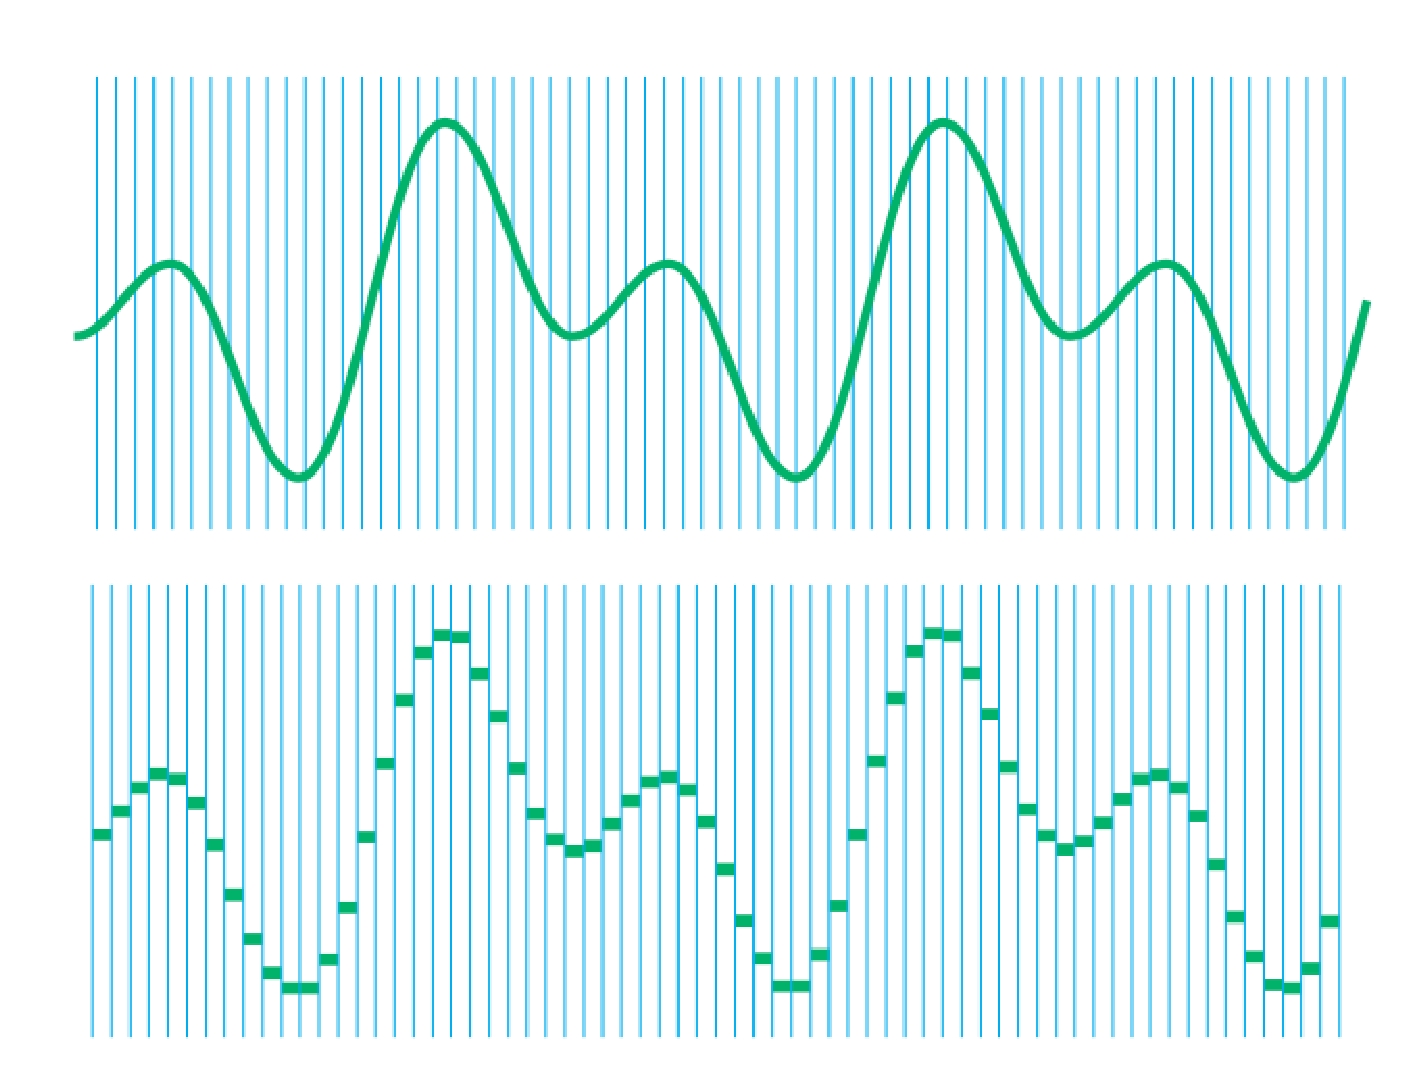
\includegraphics[width=0.7\linewidth]{bibliografia/Imagenes/transformacion.eps}
\caption{ imagen tomada de  \cite{fisica_serway}}
\label{sonido_continuo_disctreto}
\end{figure}

Posteriormente, la señal es transformada nuevamente de un espacio discreto a un espacio continuo para su correcta interpretación por parte del oído humano, este proceso trae consigo una disminución en la calidad del audio original, para estos procesos se hace necesario usar técnicas como la Transformada de Fourier y su transformada inversa. A continuación, en la figura \ref{sonido_digital} se observa el diagrama de bloque que representa el proceso de transformación de audio digital.
 
\begin{figure}[H]
    \centering
    \includegraphics[width=\linewidth]{bibliografia/Imagenes/transformacion2.eps}
    \caption{imagen tomada de \cite{audioCoding}}
    \label{sonido_digital}
\end{figure}
 
 


\subsection{Contaminación auditiva}

Este tipo de contaminación esta presente en todas las ciudades del mundo y es causada por diversos factores como la musica a volumen excesivo, el trafico, los aeropuertos, el comercio, entre otros. se considera un sonido como ruido ``cuando interfiere con actividades normales como dormir, conversar, o altera o disminuye la calidad de vida'' \cite{Agency}, estos ruidos pueden causar afectaciones a la salud\cite{ScientificAssistant1981}  ,El ministerio de ambiente de la ciudad de Bogotá ha publicado los efectos que el ruido causa en las personas \cite{Ambiente} 
\begin{itemize}
    \item{Estrés.}
    \item{Pérdida del sueño (insomnio).}
    \item{Ansiedad.}
    \item{Depresión.}
    \item{Cambios en el comportamiento (conductas agresivas).}
    \item{Baja Productividad.}
\end{itemize}
En particular y bajo la normatividad colombiana se encuentran las siguientes resoluciones relacionadas con los eventos sonoros  \cite{Ambiente}

\begin{itemize}
\item     ``Resolución No. 627/06 MAVDT: se adopta la norma nacional de emisión de ruido y ruido ambiental (parámetros permisibles, procedimientos técnicos y metodológicos para  la medición de ruido, presentación de informes, y otras disposiciones)'' \cite{Ambiente}, en esta resolución se establecen las unidades de medida para: 

\begin{itemize}
    \item[-] presión sonora: Pascal.
    \item[-] niveles de presión sonora: decibles.
\end{itemize}

También se reglamenta el uso correcto de los instrumentos de medición(sonómetro, aerómetro) así como su correcta calibración. Además se establecen los estándares Máximos Permisibles de Niveles de Ruido Ambiental como se observan a continuación.

\begin{figure}[H]
\centering
\includegraphics[width=\linewidth]{bibliografia/Imagenes/tablaNiveles2.eps}
\caption DB máximos permisibles de niveles de ruido ambiental {\cite{Ambiente}}
\end{figure}

\item     ``Resolución DAMA No. 185/99: establece condiciones generales para la obtención de permisos de perifoneo en el Distrito Capital'' \cite{Ambiente}.

\item     ``Resolución DAMA No. 832/00: establece la clasificación empresarial por impacto sonoro UCR que permite valorar las industrias y establecimientos, respecto a su nivel de generación de ruido.'' \cite{Ambiente}. 

\end{itemize}

\subsection{Inteligencia artificial en la clasificación del sonido}

En el campo de Inteligencia artificial, se han obtenido gran cantidad de logros relacionados con lo que un sistema computacional puede realizar, estos van desde máquinas que pueden competir con humanos en juegos de mesa\cite{Montesino2019}, autos que apoyan su conducción como el proyecto OpenPilot \cite{openPilot} el cual es uno de los mas importantes en el área de la conducción autónoma, análisis de información en diferentes campos por ejemplo en \cite{dornadula_credit_2019} mediante técnicas de aprendizaje de máquina se buscan patrones de comportamiento en los datos que registrados por cada una de las transacciones de compras en canales electrónicos. Así mismo, se encuentran sistemas basados en técnicas de aprendizaje de máquina para la clasificación de eventos sonoros como las diferentes técnicas de inteligencia artificial realizan un proceso similar al del cerebro humano con el fin de construir ``inteligencia". A continuación se observa como la información de archivos (datos binarios) es transformada en lo que se conoce como inteligencia 

\begin{figure}[H]
    \centering
    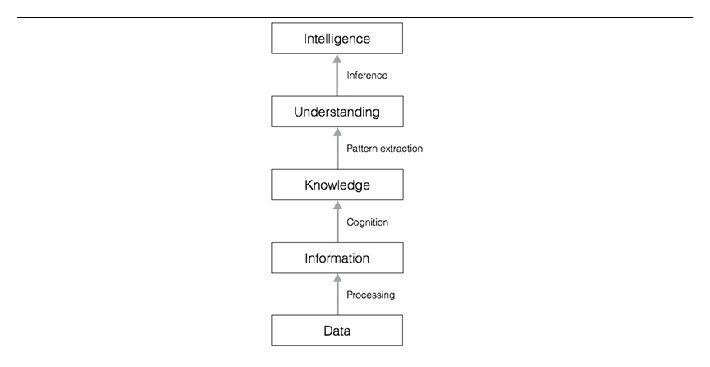
\includegraphics[width=\linewidth]{bibliografia/Imagenes/InteligenceTransform.eps}
    \caption{imagen tomada de \cite{alberto_artasanchez_artificial_nodate}}
\end{figure}

Las ramas de la inteligencia artificial se pueden clasificar de muchas maneras, en \cite{alberto_artasanchez_artificial_nodate} podemos encontrar una manera general para clasificar los diferentes algoritmos según cada aspecto relevante, un algoritmo se puede clasificar:

\begin{itemize}
    \item Según su método de aprendizaje:
    \begin{itemize}
        \item [-]    algoritmos de aprendizaje supervisados
        \item [-]    aprendizaje no supervisados
        \item [-]    aprendizaje por refuerzo
    \end{itemize}
    \item Según su función
    \begin{itemize}
        \item [-] (ANI) Inteligencia artificial estrecha: se caracteriza por realizar una tarea especifica de una muy buena manera, ratreo de paginas, juegos de mesa
        \item [-] (AGI) Inteligencia artificial General: pueden realizar cualquier tarea que un humano realiza por ejemplo conducir
    \end{itemize}
    \item Según su similitud con acciones Humanas: se caracterizan en las acciones que buscan suplir de la capacidad humana estos pueden ser 
    \begin{itemize}
        \item [-] Visión artificial
        \item [-] Aprendizaje
        \item [-] Procesadores de lenguaje natural
    \end{itemize}
\end{itemize}


Las redes neuronales artificiales son una de las técnicas mas frecuentemente usadas, estas se fundamentan una abstracción del procesamiento que realiza el cerebro humano, estas son capaces de crear un modelo con el fin de detectar los patrones presentes en un conjunto de datos y así realizar una clasificación adecuada de cada uno de los ejemplares de este conjunto. En cuanto a su arquitectura están divididas por la unión de distintas capas, se debe tener claro que una neurona es vista como la unidad mínima de procesamiento.

La neurona es la unidad básica de procesamiento dentro de una red neuronal. Cuentan con conexiones de entrada a través de los cuales reciben estímulos externos, la neurona realizará un cálculo interno y determinará una salida. 

Internamente el perceptrón realiza una suma ponderada de las entradas asignando a un valor de intensidad, también denominado peso. El cálculo interno busca que a partir de las entradas, los pesos se ajusten permitiendo determinar la salida esperada. Esto se denomina fase de entrenamiento de las neuronas. A continuación se observa la representación gráfica de una neurona.
 \begin{figure}[H]
    \centering
    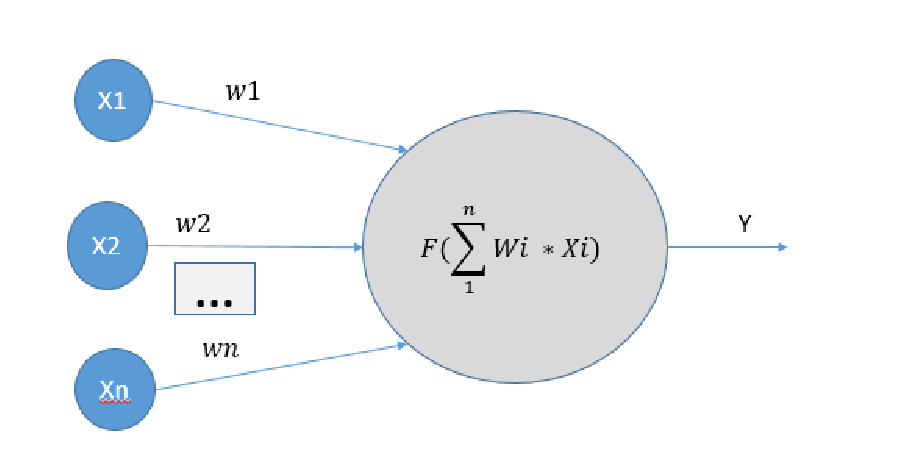
\includegraphics[width=0.8\linewidth]{secciones/Imagenes/neurona.eps}
    \caption{Neurona}
\end{figure}


Para la clasificación de audio el conjunto de datos para el entrenamiento consiste en una serie de grabaciones de eventos sonoros previamente etiquetados que ajustaran el modelo predictivo para identificar las características de los archivos de nuevos audio, finalmente basándose en las características se realiza un análisis para determinar el ejemplar a que conjunto de datos puede pertenecer.


En cuanto a los avances de inteligencia artificial como precedente encontramos el evento <<DCASE challenge>>\cite{Dc} en el cual anualmente se realiza un desafió con el fin de analizar diferentes eventos sonoros, además se encuentran los reportes técnicos de cada uno de los algoritmos implementados.\footnote{puede verse los resultados del evento del año  2020 en el siguiente enlace

\url{http://dcase.community/challenge2020/task-sound-event-localization-and-detection-results}
}.


\subsection{Arquitectura basada en Micro servicios}

En el mundo del desarrollo de software se crea la necesidad de comprender el mundo real traduciéndolo a un nivel de sistemas siempre buscando siempre un alto nivel de abstracción para esto, se utilizan diferentes enfoques como Arquitectura Orientada en servicios (SOA) o arquitectura de micro servicios. 

La arquitectura SOA busca crear sistemas por medio de conectar distintos componentes de software por medio de interfaces, esta arquitectura presenta aplicaciones mas seguras, integración con otros componente, aumento en el tiempo de entrega de los sistemas, sin embargo, esta si esta aplicación debe responder ante una gran cantidad de usuarios podría colapsar ya que es construida como una unidad (monolito),  

En la actualidad el software debe evolucionar a los cambios ágilmente. Por ejemplo, se debe responder ante una gran cantidad de usuarios o debido al dinamismo del mundo moderno la lógica del negocio se ve modificada, además de que abre la posibilidad de existencia de componentes transversales a la organización que pueden ser utilizados por diferentes áreas de negocio.

\begin{figure}[H]
    \centering
    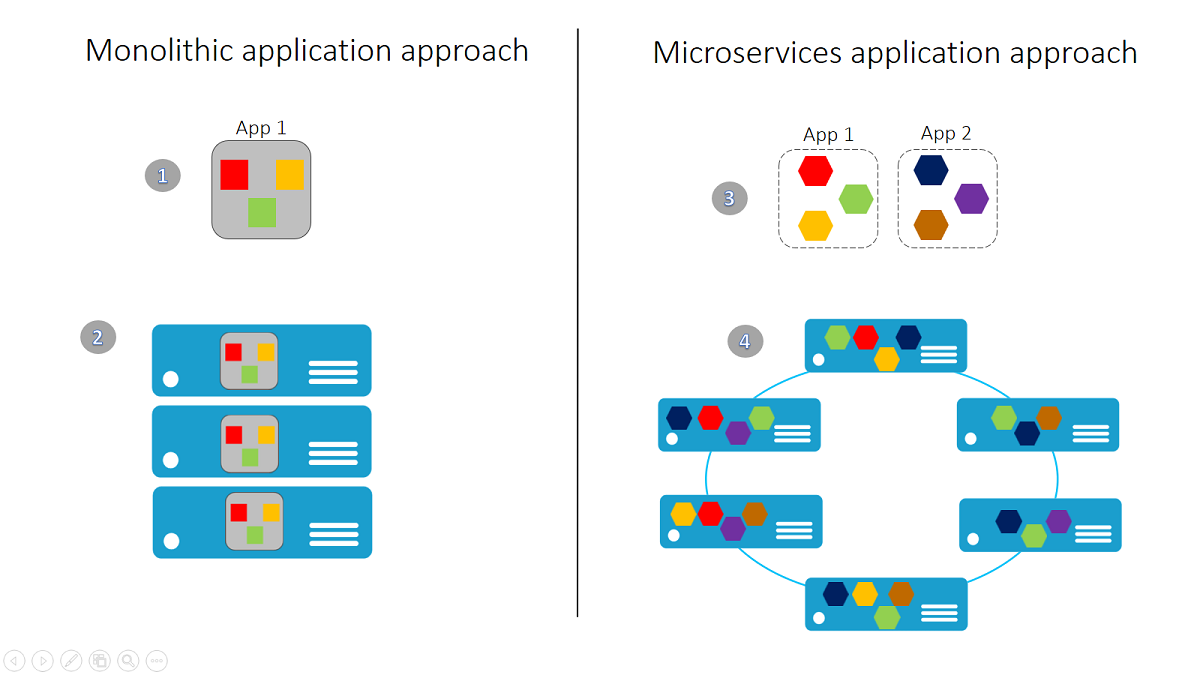
\includegraphics[width=0.8\linewidth]{bibliografia/Imagenes/monolithic-vs-micro.eps}
    \caption{imagen tomada de \cite{microservicios}}
\end{figure}


Los micro servicios presentan las siguientes ventajas frente a una arquitectura monolítica 

\begin{itemize}
    \item Se piden realizar cambios rápidamente
    \item Se implementan distintas tecnologías sin afectar el negocio, debido a que los servicios pueden ser desarrollados en  cualquier lenguaje de programación se puede elegir una tecnología adecuada para cada requerimiento
    \item Apoya la reutilización de componentes, distintas áreas del negocio pueden comunicarse para consumir un mismo servicio evitando así que cada área genere 2 veces el mismo componente.
\end{itemize}

\subsection{Arquitectura REST}

Es una arquitectura creada por Roy Fielding que define un conjunto de restricciones y principios para el diseño de sistemas distribuidos de información. De acuerdo con la página oficial de RedHat \cite{redHatREST} ``Un sistema RESTful se adhiere a las limitaciones de un estilo arquitectónico REST. Por ejemplo, la creación de una API basada en web que se adhiera a estas restricciones se considera una API web RESTful". Adicionalmente REST no esta atado a una tecnología especifica de acuerdo con Microsoft \cite{microsoftREST} ``REST es independiente de cualquier protocolo subyacente y no está necesariamente vinculado a HTTP. Sin embargo, las implementaciones REST más comunes usan HTTP como protocolo de aplicación".

Restricciones y principios, tomados de \cite{redHatREST}
\begin{itemize}
    \item La comunicación entre el cliente y el servidor debe permanecer sin estado entre solicitudes.
    \item Siempre que un servidor responde a la solicitud de un cliente, el servidor debe poder marcar esa respuesta como algo que el cliente puede almacenar en caché.
    \item interfaces uniformes.
    \item Cualquier cosa puede ser un recurso.
    \item Cada recurso debe tener un identificador único que nunca cambia.
    \item Hipermedia como motor del estado de la aplicación
\end{itemize}


\subsection{Arquitectura publicador/subscriptor}

Es una arquitectura donde los servicios pueden ejercer dos clases de funciones, publicador o subscriptor, donde el publicador anuncia eventos y el subscriptor es el encargado de procesar dichos eventos, de acuerdo a la documentación de Microsoft \cite{microsftPub/Sub} esta arquitectura ``permite que una aplicación anuncie eventos a múltiples consumidores interesados de forma asíncrona, sin acoplar los remitentes a los receptores", por lo cual esta arquitectura convertir el funcionamiento de los servicios en una coreografía. Un servicio puede comportarse como subscriptor y publicador al mismo tiempo.

Su importancia radica dependiendo del caso uso, uno de ellos es el caso cuando un servicio tiene un responsabilidad limitada al procesamiento de su propia tarea y la publicación de la misma, no requiere ni le interesa respuestas de ninguna clase, sera un procesador de eventos el encargado de mantener los demás servicios al día con las tareas pendientes publicadas y que requieran ser procesadas. La arquitectura REST por ejemplo son síncronas y por lo tanto esperan a la respuesta de una petición, en la siguiente figura se observa el patrón de arquitectura publicador/subscriptor el cual en la actualidad es la base de comunicación entre mensajes de diferentes servicios de software.

\begin{figure}[H]
    \centering
    \includegraphics[width=\linewidth]{bibliografia/Imagenes/publish-subscribe.eps}
    \caption{Arquitectura Publicador/subscriptor tomado de \cite{microsftPub/Sub}}
\end{figure}

A continuación se presentan las tecnologías que utilizan esta arquitectura
\begin{itemize}
    \item Apache KAFKA
    \item RabbitMQ
    \item ActiveMQ
    \item Redis
\end{itemize}

\subsection {Apache KAFKA}
???

\subsection{DevOps}

Son un conjunto de prácticas y filosofías que marchan en pro de la mejora continua y la entregas ágiles de acuerdo con Amazon AWS \cite{awsDevOps}. 

Las operaciones de desarrollo constituyen una combinación de filosofías culturales, prácticas y herramientas que incrementan la capacidad de una organización de proporcionar aplicaciones y servicios a gran velocidad: desarrollar y mejorar productos con mayor rapidez que las organizaciones que utilizan procesos tradicionales de desarrollo de software y administración de la infraestructura. Esta velocidad permite a las organizaciones servir mejor a sus clientes y competir de forma más eficaz en el mercado.

DevOps propone algunos principios de desarrollo: 

\begin{itemize}
    \item Desarrollo y operaciones ya no están aislados.
    \item Los equipos de control de calidad y de seguridad se integran.
    \item Equipos utilizan prácticas para automatizar los procesos que anteriormente habían sido manuales y lentos (implementar código o aprovisionar infraestructura, etc).
\end{itemize}

Beneficios de DevOps:

\begin{itemize}
    \item Velocidad y adaptación al cambio.
    \item Aumento en la frecuencia de entregas.
    \item Confiabilidad.
    \item Incremento en capacidad de escalado.
    \item Mejora en la colaboración, comunicación he integración de equipos.
    \item Mejora en la seguridad.
\end{itemize}

\subsection{Integración continua / Entregas continuas}

DevOps propone ciertas prácticas de desarrollo que buscan la agilidad por medio de la automatización de procesos, existen procesos claves para lograr el objetivo el primero de ellos la Integración continua que de acuerdo con Amazon AWS \cite{awsIC} ``es una práctica de desarrollo de software mediante la cual los desarrolladores combinan los cambios en el código en un repositorio central de forma periódica, tras lo cual se ejecutan versiones y pruebas automáticas", las pruebas que constantemente verifican que los desarrollos sean afines a la funcionalidad esperada y evitan posibles fallas en nuevos desarrollos. El segundo componente son las entregas continuas o despliegues continuos (difieren en que el despliegue final debe ser autorizado en el caso de entregas continuas), buscan automatizar el proceso de gestión de recursos y despliegue de código para la fase productiva, de acuerdo con Amazon AWS \cite{awsEC} la entrega continua ``es una práctica de desarrollo de software mediante la cual se preparan automáticamente los cambios en el código y se entregan a la fase de producción".

\begin{figure}[H]
    \centering
    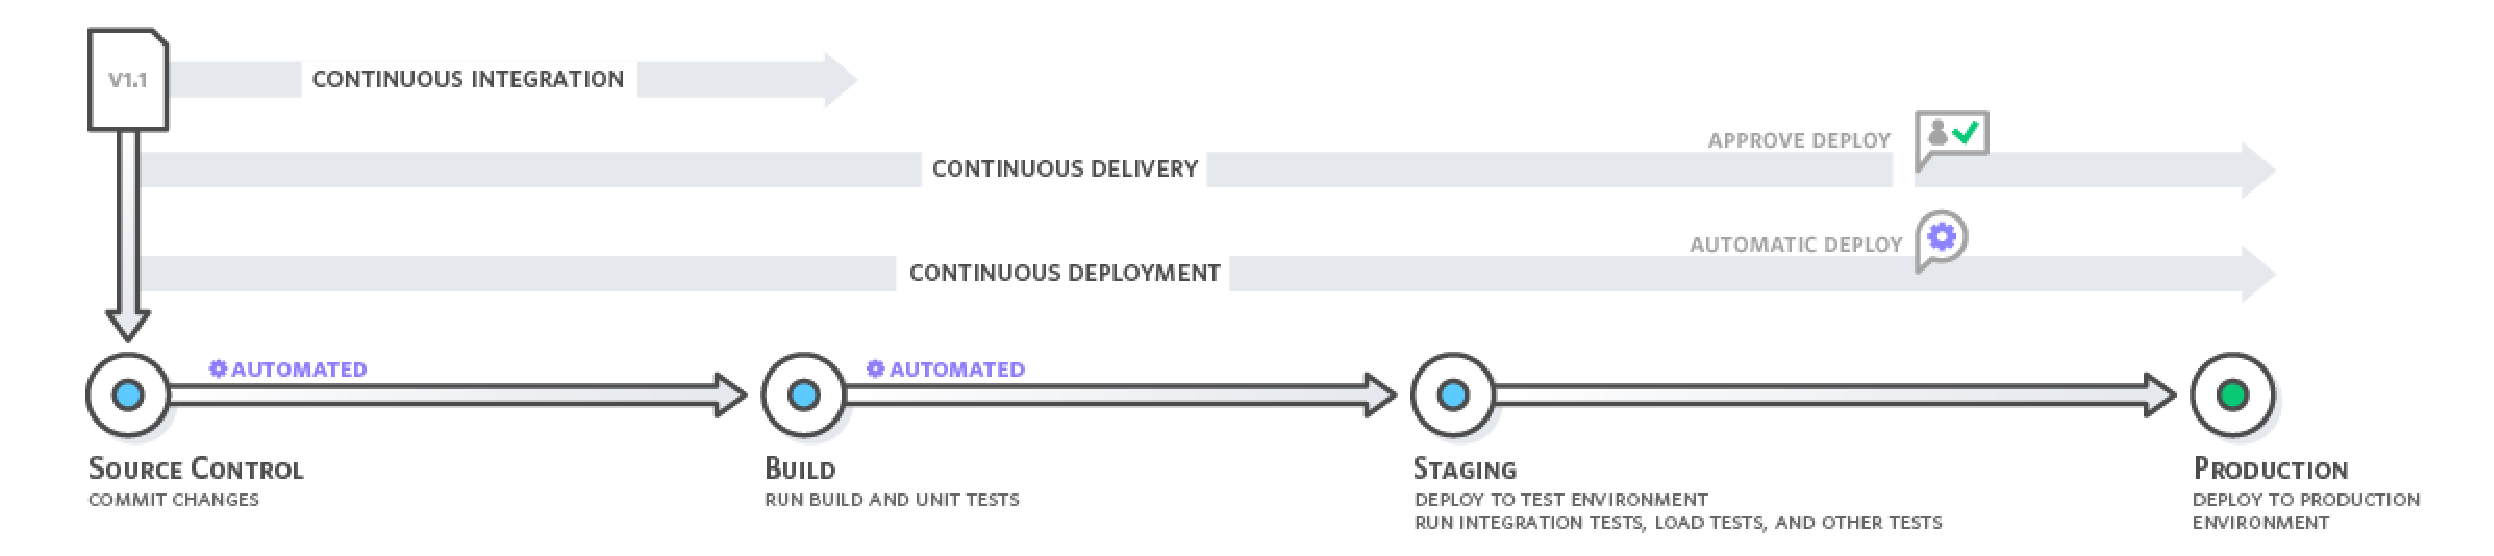
\includegraphics[width=\linewidth]{bibliografia/Imagenes/awsEC.eps}
    \caption{Diagrama de entregas continuas, tomado de \cite{awsEC}}
\end{figure}

Para lograr el objetivo de la integración continua y las entregas continuas existen diversas herramientas, dando mención a algunas estas son:

\begin{itemize}
    \item Terraform (Aprovisionamiento de infraestructura)
    \item CircleCI
    \item TravisCI
    \item Jenkins
    \item AWS Pipeline
\end{itemize}

\subsection{Versionamiento semántico}

Es un conjunto de reglas definidas para el control de versiones de un software y sus dependencias, que permite observar a grandes rasgos cambios y consecuencias al momento de definir o actualizar una dependencia, de acuerdo al autor Tom Preston-Werner en la web oficial \cite{semver} las reglas permiten definir:

Cómo asignar y cómo aumentar los números de versión. Para que este sistema funcione, tienes que declarar primero un API pública. Esto puede consistir en documentación o ser explicitado en el código mismo. De cualquier forma, es importante que esta API sea clara y precisa. Una vez que identificaste tu API pública, comunicas cambios a ella con aumentos específicos al número de versión. Considera un formato de versión del tipo X.Y.Z (Major.Minor.Patch) Los arreglos de bugs que no cambian el API incrementan el patch, los cambios y adiciones que no rompen la compatibilidad de las dependencias anteriores incrementan el minor, y los cambios que rompen la compatibilidad incrementan el major.

Este tipo de prácticas permiten evitar caer en dos problemas definidos por el autor, el primero el bloqueo de versiones (no se puede actualizar una pieza de software sin tener que actualizar todos los que dependen de la misma) o promiscuidad de versiones (asumir más compatibilidad con versiones futuras de lo razonable). Las reglas así mismo están documentadas en la web oficial.

\subsection{CircleCI}

CircleCI \cite {circleci} es una plataforma de CI/CD en la nube para la automatización de canales. Desde la interfaz de CircleCI se pueden pueden asociar repositorios de  GitHub. La el flujo de un canal es definida en un archivo de configuración YAML.

A continuación se definen algunos conceptos fundamentales para construir un canal en circleCI:

\begin{itemize}
	\item Step(Paso): Un comando que se ejecuta dentro de un trabajo.
	\item Job(Trabajo): Conjunto de pasos que se ejecutan en una sola unidad (un contenedor, una máquina).
	\item Workflow(Canal): Orden de los trabajos con sus respectivas reglas de ejecución.
\end{itemize}

\begin{figure}[H]
	\centering
	\includegraphics[width=\linewidth]{bibliografia/Imagenes/job.PNG}
	\caption{Un boceto de la configuración de un trabajo para pruebas unitarias}
	\label{jobcircle}
\end{figure}

Un trabajo requiere un conjunto de pasos y un contenedor (donde se ejecutan todos los pasos), como se ve en la figura \ref{jobcircle} ``Test'' es un trabajo que prepara la máquina y ejecuta las pruebas unitarias. La falla o interrupción de un trabajo detiene el flujo del canal (o flujo de trabajo) y es notificado en la interfaz de circleCI y Github para evitar su integración.

\begin {figure} [H]
\centering
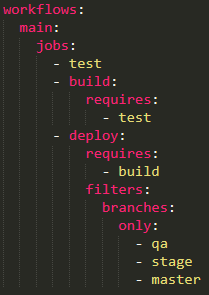
\includegraphics [width=0.5\linewidth]{bibliografia/Imagenes/workflow.PNG}
\caption{Ejemplo de un flujo de trabajo}
\label{workflow}
\end {figure}

En la figura \ref{workflow} se define un flujo de trabajo en el cual se definen una serie de filtros y atributos para determinar el orden y los pasos por cada rama

\subsubsection {Orb}

CircleCI \cite {circleci} define orb como ``fragmentos de código reutilizables que ayudan a automatizar los procesos repetidos''. Orbs permite reducir los pasos y la configuración simplemente llamando a un trabajo determinado (ya definido en el orb) en el flujo de trabajo agregando solo atributos adicionales, filtros o variables de entorno si es necesario. Como resultado, los orbes reducen la complejidad en una configuración y el tiempo para implementar nuevos flujos de trabajo en un canal.

\begin{figure}[H]
	\centering
	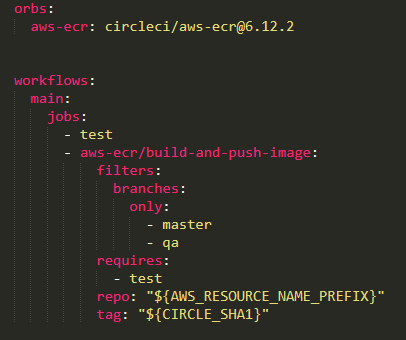
\includegraphics [width=0.4\linewidth]{bibliografia/Imagenes/orbexample.PNG}
	\caption {Ejemplo de la configuración de un orb}
	\label{orbexample}
\end{figure}

Los orb se definen en el atributo ``orbs'' en el archivo YAML del círculo CI. Un ejemplo es el orb ``aws-ecr/build-and-push-image'' que se usa en cuando se debe construir una imagen y subirla a AWS ECR (Elastic Container Registry), como se ve en la Figura \ref{orbexample}, no es necesario crear un trabajo ni escribir ningún comando, solo se necesitan los atributos necesarios para funcionar. Sin este orb, se deben agregar pasos adicionales como la instalación de AWS CLI y todo el proceso de creación de imágenes.

\subsection {IAC}

Matej Arta \ v {c} et al. definir una relación entre DevOps y la infraestructura como código (IaC):

\leftskip1.27cm\relax
\rightskip1.27cm\relax

DevOps promueve el uso de una noción típica de desarrollo de software, es decir, ``código fuente'', también para diseños de infraestructura, de modo que todo el conjunto de scripts, código de automatización y configuración, modelos, dependencias requeridas y parámetros de configuración operativa se pueden expresar utilizando el mismo idioma estándar. \cite{devopsiac}

\leftskip0cm\relax
\rightskip0cm\relax

IaC se encarga de todas las operaciones de la infraestructura (creación, actualización y eliminación) utilizando una definición de los recursos sin la intervención de desarrolladores o miembros de operaciones, por lo que ambos solo necesitan monitorear el estado de implementación o ser notificados si fue exitoso o no.
Terraform \cite{terraform} es una herramienta para IaC y utiliza una sintaxis para configuraciones que se llama HashiCorp Configuration Language (HCL), con esta sintaxis es posible describir la infraestructura en Amazon Web Services, Azure, Google Cloud, Kubernetes y otros proveedores.

\subsection {Terraform}
\subsubsection {Recursos}
\subsubsection {Varibles}
\subsubsection {Modulos}
???
\subsection {SonarCloud}
???
\subsection {AWS}
???
\subsubsection {ECR}
???
\subsubsection {S3}
???
\subsubsection {ECS}
???
\subsubsection {Servicio}
???
\subsubsection {Definición de tarea}
???
\subsubsection {CloudWatch}
???
\subsubsection {Lambda}
???
\subsubsection {VPC}
???
\subsection {ElasticStack}
???
\subsubsection {Logstash}
???
\subsubsection {ElasticSearch}
???
\subsubsection {Kibana}
???